\documentclass{sigcomm-alternate}

\begin{document}

\title{Net Neutrality, Bandwidth Usage and Government Regulations}
	
\numberofauthors{3}

\author{
	% 1st. author
	\alignauthor
	Raz Friman\\
	\affaddr{Southern Methodist Univeristy}\\
	\affaddr{5600 SMU Blvd. APT 1516}\\
	\affaddr{Dallas, Texas, 75206}\\
	\email{rfriman@smu.edu}
	% 2nd. author
	\alignauthor
	Jarret Shook\\
	\affaddr{Southern Methodist Univeristy}\\
	\affaddr{5555 Amesbury Dr. APT 1303}\\
	\affaddr{Dallas, Texas, 75206}\\
	\email{jshook@smu.edu}
	% 3rd. author
	\alignauthor Elena Villamil\\
	\affaddr{Southern Methodist Univeristy}\\
	\affaddr{5555 Amesbury Dr. APT 1303}\\
	\affaddr{Dallas, Texas, 75206}\\
	\email{mvillamilrod@smu.edu}
	\and  % use '\and' if you need 'another row' of author names	
	% 4th. author
	\alignauthor Jeffrey Artigues\\
	\affaddr{Southern Mehthodist University}\\
	\affaddr{9520 Amberton Pkwy.}\\
	\affaddr{Dallas, Texas, 75243}\\
	\email{jartigues@smu.edu}
}

\maketitle

\begin{abstract}
This paper focuses on the impact of laws enforcing Net Neutrality and the regulation of the Internet as a utility. Net Neutrality is a widely debated technical topic that is being discussed politically because its implementation affect a significant range of individuals and companies.  The political discussions broaden the topic to focus on more than just the technical aspects; the current discussions include the economical, political and technical impacts of Net Neutrality. In this paper, we explore how bandwidth usage is affected by Net Neutrality, how prioritization affects the network, how other countries that have implemented Net Neutrality compare to the US, and the economic and business implications of Net Neutrality. 
\end{abstract}



\section{Introduction}
In February 2014, Netflix issued a class action lawsuit against Comcast stating that it was illegal for Comcast to throttle back Netflix speeds due to bandwidth usage. The lawsuit ended with Netflix settling out of court with Comcast. This lawsuit was a big motivation for reviewing regulations on Internet, not just in the US but also in Europe. Europe has already approved regulations that protect Net Neutrality along with Japan. Furthermore, two of the main foci of the latest bill passed by the FCC are to establish Net Neutrality and to regulate the Internet as a utility based on the 1934 telecom bill. The question is: how do these laws, in particular regulating Internet as a utility, politically and economically affect the country, and how do they affect the quality of service of the Internet?

First, we define Net Neutrality as: “the principle according to which all Internet traffic is treated equally, without discrimination, restriction or interference, independently of its sender, recipient, type, content, device, service or application”\cite{gigaom}. In our research we start by analyzing current network traffic, and then we draw conclusions on how Net Neutrality would affect this usage. Network traffic is significantly increasing, and in particular video streaming is the service increasing most rapidly \cite{cisco}. As of today, with the way Internet is being regulated, this bandwidth usage is not a problem. However, if we add in the idea of Net Neutrality and stricter limitations on what ISPs can do, then the quality of service may suffer.  For example, imagine that the Internet is a system of highways. If we allow all packets to travel in the same way without traffic enforcement (throttling), could we lose performance over the network as a whole? \cite{tandlInfographic}

Next, we examine the new bill passed by the FCC to regulate the Internet under Net Neutrality as a utility. As of the time of writing the bill is not publically available, therefore we will be analyzing the bill’s utility aspect which has been explained to apply the 1944 telecom bill.  By analyzing this bill we will show what legal rights the government has in applying regulations to Net Neutrality with this bill. This bill marks a large change for the US in several different aspects. First, it has economical effects for the ISPs, the consumers, and the government. For example, ISPs like Comcast and Verizon will lose the money from any agreement they had made with companies like Netflix.  Thus, to compensate for their losses, they may increase their customer prices, which will adversely affect the customer \cite{inthenews}. Additionally, taxes may also increase the amount the end user will have to pay for Internet services. Second, it may affect the performance (Quality of Service) of Internet. Meaning will the Internet’s speed be hurt because ISPs will not be able to regulate the traffic in the same way? Third, it has political effects; simply because this bill may incur taxes and obviously, gives government control to regulate the internet in accordance to the 1944 Telecom Bill. Lastly, we will compare our findings of Net Neutrality in the US with Internet regulation implementations in Europe and Japan.

The following sections are organized as follows: first, with an analysis of the current Internet bandwidth usage. Next we provide an overview of the current bill passed by the FCC by analyzing the 1944 Telecom Bill. In a later section we will discuss its different political, economical and technical implications. Afterwards, we discuss Net Neutrality in Japan and Europe and its relation to the US.


\section{Related Work}
There is an ever-growing collection of publications, articles, and news reports about Net Neutrality. Unfortunately, almost all of these sources usually include some degree of bias in them. In order to get unbiased information about this topic, we have to analyze multiple sources with all levels of bias from different sides and combine their information together to get a better understanding of Net Neutrality and Internet regulations. This includes reading White Papers published by major ISPs in addition to the articles published by the FCC favoring their Net Neutrality proposal. By pairing both sides of heavily biased sources, we can extract the relevant information and create a view that is less biased towards either side. 

We also reviewed the laws and regulations in effect in Europe and Japan where Net Neutrality is already established. In the next section, we compare these regulations with the new regulation passed in the United States and analyze how they relate and how they differ. Finally, we also analyze research papers discussing different economic ramifications and the effects of Net Neutrality and its regulations in business. 


\section{Research Approach}

\subsection{Bandwidth Usage}
As we transition into an even more interconnected world with the Internet of Things, real time information most likely in small quantities is expected to be in high demand and readily available \cite{cisco}. Streaming services like Netflix still continues to dominate the global amount of network traffic\cite{Sandvine}. usage on the Internet is constantly evolving, and the infrastructure supporting the Internet needs to be able to adapt to these changes. According to Cisco’s annual VNI report, video streaming currently accounts for over 60\% of traffic usage on the Internet \cite{cisco}. Using current projections and traffic analysis, they predict that within 5 years, video streaming will grow to account for over 80\% of traffic usage. This is a huge amount of data that must seamlessly be transported across the world. If the current infrastructure is not set up and managed correctly, there will be drastic consequences. One issue regarding how ISPs handle this massive growth in demand has already occurred, and the solution was not very elegant.

Between 2013 and 2014, before any FCC proposals of Net Neutrality were introduced, Netflix and Comcast got into an argument over bandwidth usage\cite{netflix}. With the growing use of video streaming, Netflix, was taking up more and more bandwidth from ISPs. When an ISP’s bandwidth is congested from Netflix streaming, there is less room to transmit other types of traffic. In order to remediate this issue, Comcast demanded a fee from Netflix for using up a majority of its bandwidth. At the same time, it used this excuse to begin throttling back Netflix traffic in order to allow more room for other types of traffic. Netflix stated that this sort of action was unfair and against the basic principles of Net Neutrality; therefore, they went to court to solve their issues. As the court proceedings continued, Comcast continued to throttle back Netflix’s bandwidth speed further and further. Eventually, in February of 2014, Netflix and Comcast settled out of court and Netflix paid Comcast an undisclosed amount under a peering agreement. As soon as this agreement was reached, Netflix’s speed on Comcast’s network went up over 45\% within 2 months. Afterwards, Verizon took advantage of this situation by demanding a premium from Netflix as well. As Netflix’s customers complained about slowing speeds, Netflix had no choice but to pay the fee in order to restore its customers’ expected quality of service. The bandwidth speeds for Netflix on both Comcast and Verizon can be seen on Figure \ref{fig:netflix} below. Figure ~\ref{fig:netflix} demonstrates that as soon as an agreement was reached, the bandwidth throttling ceased and returned to normal speeds.

These actions demonstrate a flaw in fair competition that Net Neutrality has the potential to fix. If these negotiations and agreements continue to form, ISPs like Comcast and Verizon will be able to charge both the customers and content providers for using bandwidth. Additionally, this will give larger companies an unfair advantage in gaining more access to bandwidth as compared to small business and startups. A system that supports large corporations and makes competition with smaller businesses impossible is harmful to consumers and creates a large barrier of entry for all Internet-related businesses.

\begin{figure}
	\label{fig:netflix}
	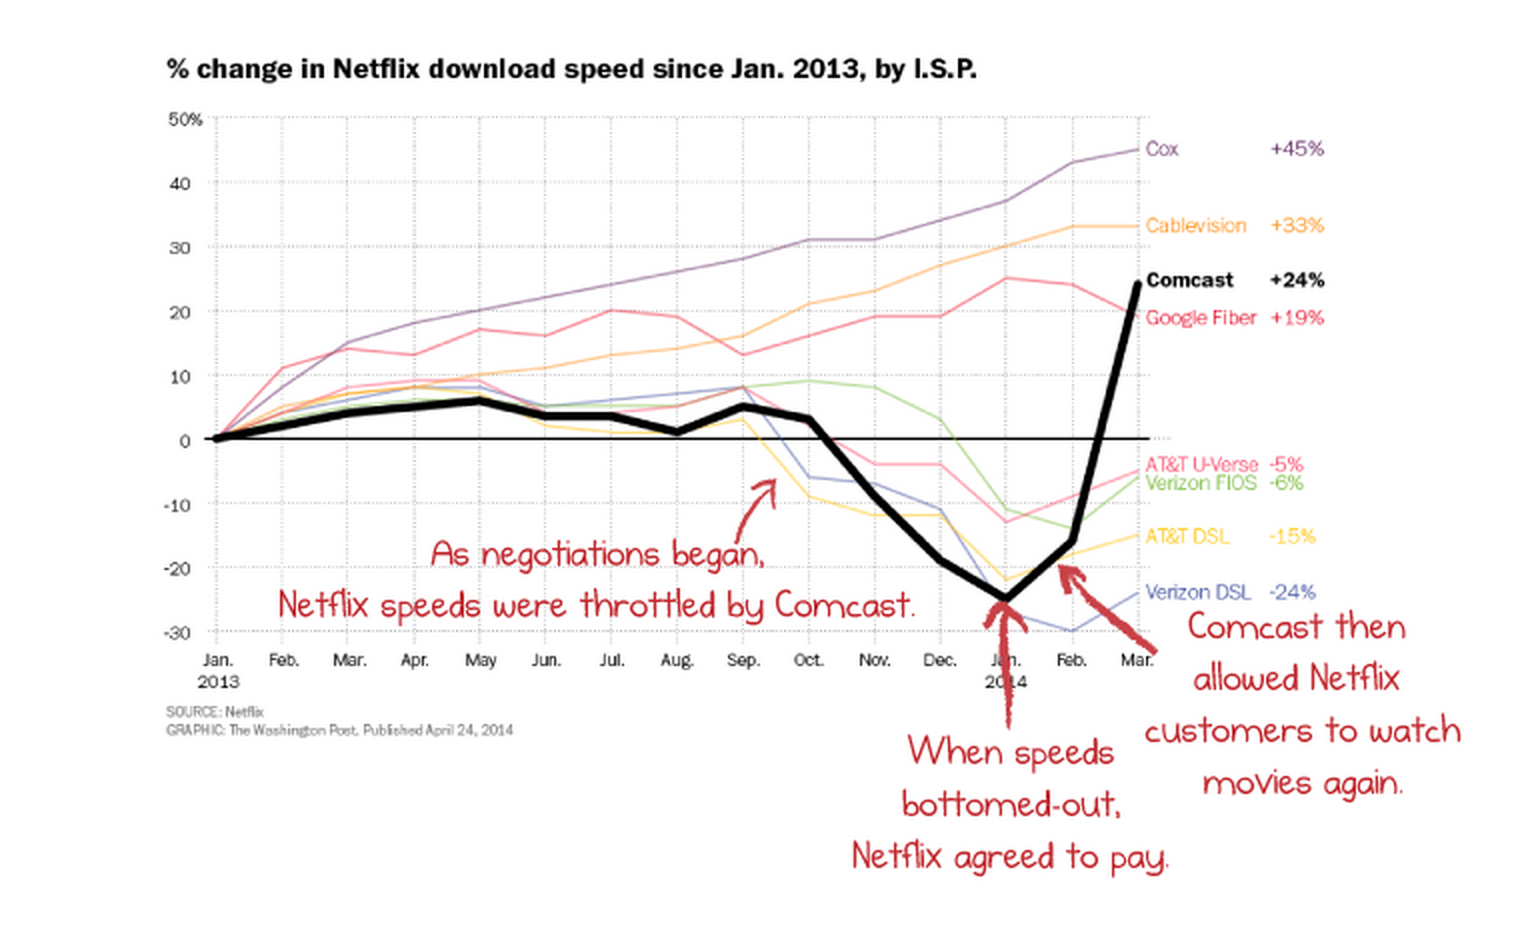
\includegraphics[scale=.20]{NetflixGraph.png}
	\caption{Graph comparing Netflix bandwidth speeds over time from different ISPs.}
\end{figure}


\subsection{Net Neutrality in Europe}

In September of 2013, the European Commission (EC) proposed the European Union’s new package of telecom laws. This package included the Net Neutrality legislation. With this legislation the EC aimed to protect Net Neutrality in the European Union (EU) and to stop the “blocking or throttling of competing or data-heavy sources” \cite{economics}. However, this legislation also gives ISPs the freedom to offer higher speeds or quality for specialized services as long as the standard Internet is not harmed by it \cite{economics}.

In April of 2014 the European Parliament voted and passed the telecom law reform proposed by the EC. They did add some amendments to properly define and protect Net Neutrality, notably amendments 235 and 236. Amendment 235 gives a strong definition of “specialized services”, the goal of this amendment is to give ISPs strong constraints to what they can consider outside standard Internet. Amendment 236 specifies that this specialized services shall only be provided if the network has capacity enough to support standard services plus the specialized services without any detrimental result on the quality of Internet. In addition this amendment also determinants that providers cannot discriminate between equivalent services and applications \cite{gigaom}.

These reforms happened soon after the Netflix deal with Comcast and Verizon was approved in United States. In particular, The fact that amendment 235 gives a strong definition of “specialised services”  keep ISPs from putting into this category services that do not belong there, such as Netflix, in order to get extra money from them\cite{gigaom}.

David Meyer, European correspondent for tech site Gigaom, has an interesting opinion on the new regulations and on Net Neutrality in Europe versus United States. According to him, the new laws will allow European consumers to be in control. He also claims that ISPs will not be able to raise the costs because of the existence of a high competitive market, meaning that if ISPs dramatically increase their prices then they will lose customers*. Moreover, he also believes that in the US, ISPs can degrade services that do not match their interests, and this is not in the interest of the consumer. He also affirms that new entrants into the the US market could be disadvantaged because they do not have enough money to pay ISPs \cite{inthenews} \footnote{Meyer refers this part specifically to UK, but we believe it can be applied to Europe in general.} .

In conclusion, the EU has Internet regulations that enforce Net Neutrality, and that restrict ISPs’ range of action. However, none of these regulations mention regulating Internet as a utility. It is important to note that it is not entirely fair to straight out compare the EU with the US since there are a lot of different characteristics that make them unique. However, the fact that Europe is working under Net Neutrality laws without utility or pricing regulations, and that the ISPs in Europe have not had any problems providing consumers with good quality Internet, is a very important fact to take into account.



\subsection{Net Neutrality in Japan}

Japan, in comparison to the EU, has had Net Neutrality for a longer period of time.  They make a good case study to how effectively their country has been able to handle bandwidth congestion.  Most importantly, Japan differs from the United States in that there is more ISP competition\cite{jitsuzumi2011japan}.  This is guaranteed by regulations from the government as there are certain companies which are unable to grow past the point they are.

As previously explained, if there ever is a situation where 100\% of a network is used, all packets being sent inside the network past that point would be dropped.  People would experience loss of service, dramatic slowdowns and general unusability.  Because all Internet traffic must be treated equally in a Net Neutral environment, there is no way to individually contain users who may be using the largest portion of traffic.  For example, if there ever was a case in which a company was using 80\% of the network, it makes little sense to throttle back every user of that network when the majority of the network could be unaffected by throttling that one company.  With that said, this is not possible under Net Neutrality laws, as you would not be giving equal treatment to everyone on the network.

Japan, addressing this problem has set a few different things into place.   Specifically, Japan’s main response with how to combat this potential problem is by pushing ISPs to improve infrastructure. Important to note, the country has never experienced a “blackout” or reached 100\% network usage.  Therefore, so far their strategy has been successful.  However, they have come close, specifically in 2007 90\% of the entire Japanese download bandwidth was used, with 80\% of its upload bandwidth being used during peak hours\cite{jitsuzumi2011japan}.



\subsection{Economic and Business Implications}

A major concern of shifting to a Net Neutral environment is the potential for regulations to stifle the innovation and development that the Internet is known for. Competition naturally leads to developments, as companies are constantly fighting each other for customers, and ISPs are no exception. The move towards a net neutral Internet could have negative implications for the development of new technologies and improvements to the existing networks. Without monetary incentive, ISPs will certainly be less inclined to provide and maintain services beyond what it is required. On the other hand, the opposite argument can also be made. In the US there are cases where customers only have access to one or two ISPs; therefore, the motivation for companies to provide the best for customers does not exist. Instead they will only be motivated to  stay ahead of local competition.  Thus, the limited options due to a lack of competition in those areas also results in the stagnation of innovation \cite{Crowcroft:2007:NNT:1198255.1198263}.

The economic feasibility of supporting a net neutral Internet is also something that must be considered. Net Neutrality requires that all traffic be treated equally. According to this principle, a few users maxing out a shared pipeline’s bandwidth capacity with something data intensive like video streaming would result in everyone using that pipeline having their data transfer throttled. A related issue is the potential for all users to have high data transfer rates simultaneously. The current infrastructure already has issues even with throttling, thusand without significantly improving the existing infrastructure it would become even more of a problem. However as mentioned previously, the desire for companies to invest in the infrastructure is expected to decline, making it even less likely that such a change would be encouraged.
\cite{paradox}



\bibliographystyle{unsrt}
\bibliography{bib}

\end{document}
